\documentclass{math}

\usepackage{float}
\usepackage{graphicx}
\usepackage{listings}
\usepackage{subcaption}

\title{Principles of Data Management}
\author{Insert Group Name Here}
\date{August 2018 - December 2018}

\begin{document}

\lstset{basicstyle=\ttfamily\footnotesize,breaklines=true}
\maketitle

\section*{Phase 2}
Our application software will be in the form of a command line interface that
provides a tree of commands to the user. The intended user of this software will
be administrators who can access information related to customers, dealers,
vehicles, and the relationships between them. This software can also function
as an abstraction of the database to developers who need access to a higher
level API that can provide information about the relationships between
customers, dealers, and vehicles.

\subsection*{ER Diagram}

\subsection*{Application Software}
The user interface will be a command line interface using a tree of commands
that allow access to customers, dealers, vehicles, and information related to
the relationships between them.
\begin{figure}[H]
  \centering
  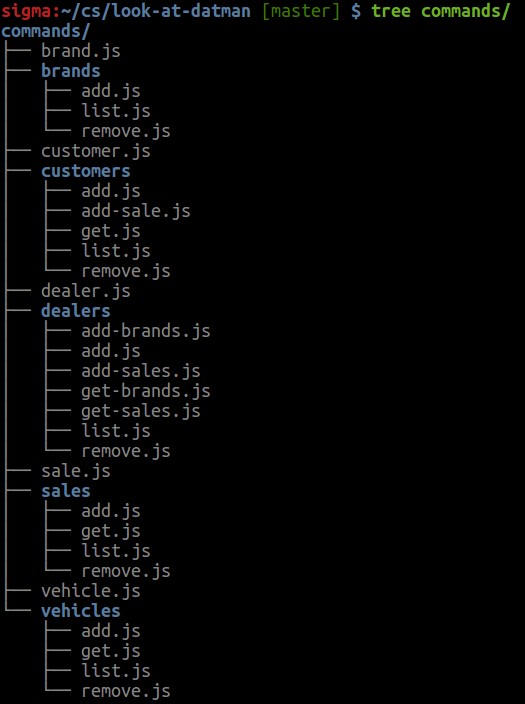
\includegraphics[width=8cm]{assets/phase2_command_tree.png}
  \caption{Minimal command tree of available actions}
\end{figure}
\begin{figure}[H]
  \centering
  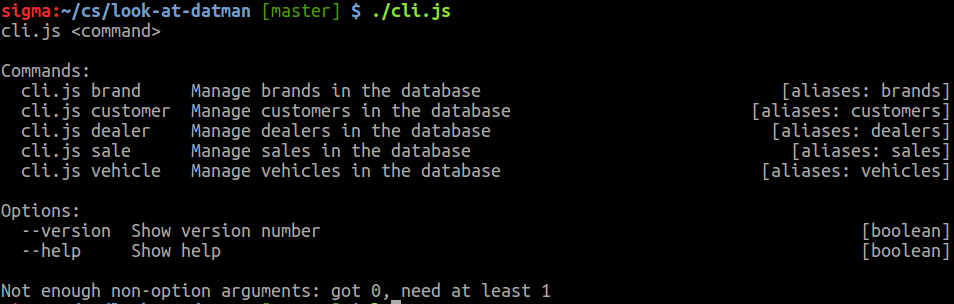
\includegraphics[width=16cm]{assets/phase2_manpage.png}
  \caption{CLI help prompt}
\end{figure}
The CLI will internally handle formatting and assembling more complicated
queries before executing it on the database. It will directly query the database
with relevant queries to fetch data for display. The user-facing input side of
the software (argument capturing, command line flags, command tree) is handled
by the \texttt{yargs.js} package while the table display formatting is handled
by the \texttt{cli-table3} package (both available on npmjs).

\subsection*{Sample SQL}
Creating the tables:
\begin{lstlisting}
create table if not exists customer (
  id int primary key,
  income int,
  name varchar(255),
  phone varchar(255),
  gender varchar(16),
  address_street varchar(255),
  address_state varchar(255),
  address_zipcode varchar(255)
);

create table if not exists dealer (
  id int primary key,
  name varchar(255),
  phone varchar(255)
);

create table if not exists brand (
  name varchar(255) primary key,
  country varchar(255),
  reliability varchar(255)
);

create table if not exists sale (
  id int primary key,
  customer int references customer(id),
  dealer int references dealer(id)
);

create table if not exists vehicle (
  vin int primary key,
  model varchar(255),
  transmission varchar(255),
  mileage int,
  engine varchar(255),
  color varchar(255),
  brand varchar(255) references brand(name),
  dealer int references dealer(id),
  sale int references sale(id),
  customer int references customer(id)
);

create table if not exists brand_dealer (
  brand varchar(255) references brand(name),
  dealer int references dealer(id)
);
\end{lstlisting}
Fetching all vehicles purchased by a customers in NY:
\begin{lstlisting}
select model,brand from vehicle where customer in
  (select id from customer where address_state = "NY");
\end{lstlisting}
Set a brand's reliability:
\begin{lstlisting}
update brand set reliability="poor" where name="Ford";
\end{lstlisting}
Add a new vehicle for a dealer:
\begin{lstlisting}
insert into vehicle values(
  1243, "Accord", "Automatic", 10000, "V6", "Ugly", "Honda", 3, NULL, NULL)
\end{lstlisting}

\subsection*{User Interface}
If a query is executed via the command line, the data returned will be nicely
formatted into a terminal compatible table for display.
\begin{figure}[H]
  \centering
  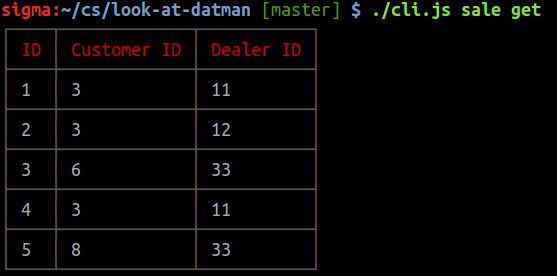
\includegraphics[width=10cm]{assets/phase2_example_table.png}
  \caption{Formatted table in terminal}
\end{figure}

\subsection*{Sample Data}
Included in the project zip as CSVs.

\begin{center}
  You can find all my notes at \url{http://omgimanerd.tech/notes}. If you have
  any questions, comments, or concerns, please contact me at
  alvin@omgimanerd.tech
\end{center}

\end{document}
